\documentclass{article}

\usepackage{makeidx}  % allows for indexgeneration
\usepackage{mathtools} %
\usepackage{graphicx} %
\usepackage{xcolor}
\usepackage{subfig}
\usepackage{caption}
%\usepackage{makecell}
%\usepackage{subcaption}
\usepackage{amsmath}
\usepackage{amsthm}
\usepackage{amssymb}
\usepackage{xspace}
%\usepackage{multirow}
%\usepackage{comment}
%\usepackage{secdot}

\newtheorem{problem}{Problem}

\title{Modeling Time-series gene expression data by a non-redundant set of time points}

\begin{document}

\maketitle

\section{Problem Formulation}

Let $D$ be the time series data at time points $t \in T$ for set of genes $g \in G$ where $d_{g}^{t}$ is the expression value of gene $g$ at time point $t$. We are interested in solving the following problem:

\begin{problem}
Given time-series gene expression data $D$ over set of $T$ time points and number of time points $k$, we try to find the best $k$-subset of all time points which can reconstruct the whole expression data as accurately as possible.
\end{problem}

\section{Results}

\subsection{Mean Squared Error over selected number of points}\label{sec:errtime}

When using the weighting scheme, we run k-means with increasing number
of clusters and select the number of clusters as $8$ by BIC. We also
estimate the number of clusters by $\sqrt{\frac{n}{2}}$ which is also
$8$. Cluster sizes are $1$, $40$, $11$, $12$, $45$, and $25$. Figure~\ref{fig:fig1}
shows the mean squared error over time for both unweighted and
weighted cases as well as the following two initial conditions: 1-
\textit{Equal Partition Heuristic}: We partition the time points
almost equally so that each interval will have almost equal number of points, 2- \textit{Maximum Absolute Difference Heuristic}: We sort the points by the average absolute difference between
its consecutive neighbours, and select the first $k$ points as our initial solution where $k$ is the number of required points. We also
report the results from simulated annealing which does not always select the optimum solution but instead it selects suboptimal solutions depending on the temperature.

Selected time points for weighted case is: [0.5, 1.0, 1.5, 2.5, 3.5, 5.5, 6.5, 8.5, 10.5, 12.0, 16.0, 18.0, 22.0, 24.0, 27.0]

Selected time points for unweighted case is: [0.5, 1.0, 1.5, 2.5, 3.5, 6.5, 8.0, 8.5, 10.5, 12.0, 13.0, 15.0, 19.0, 24.0, 27.0]

Selected time points for weighted and unweighted cases match closely.

\begin{figure}
\centering
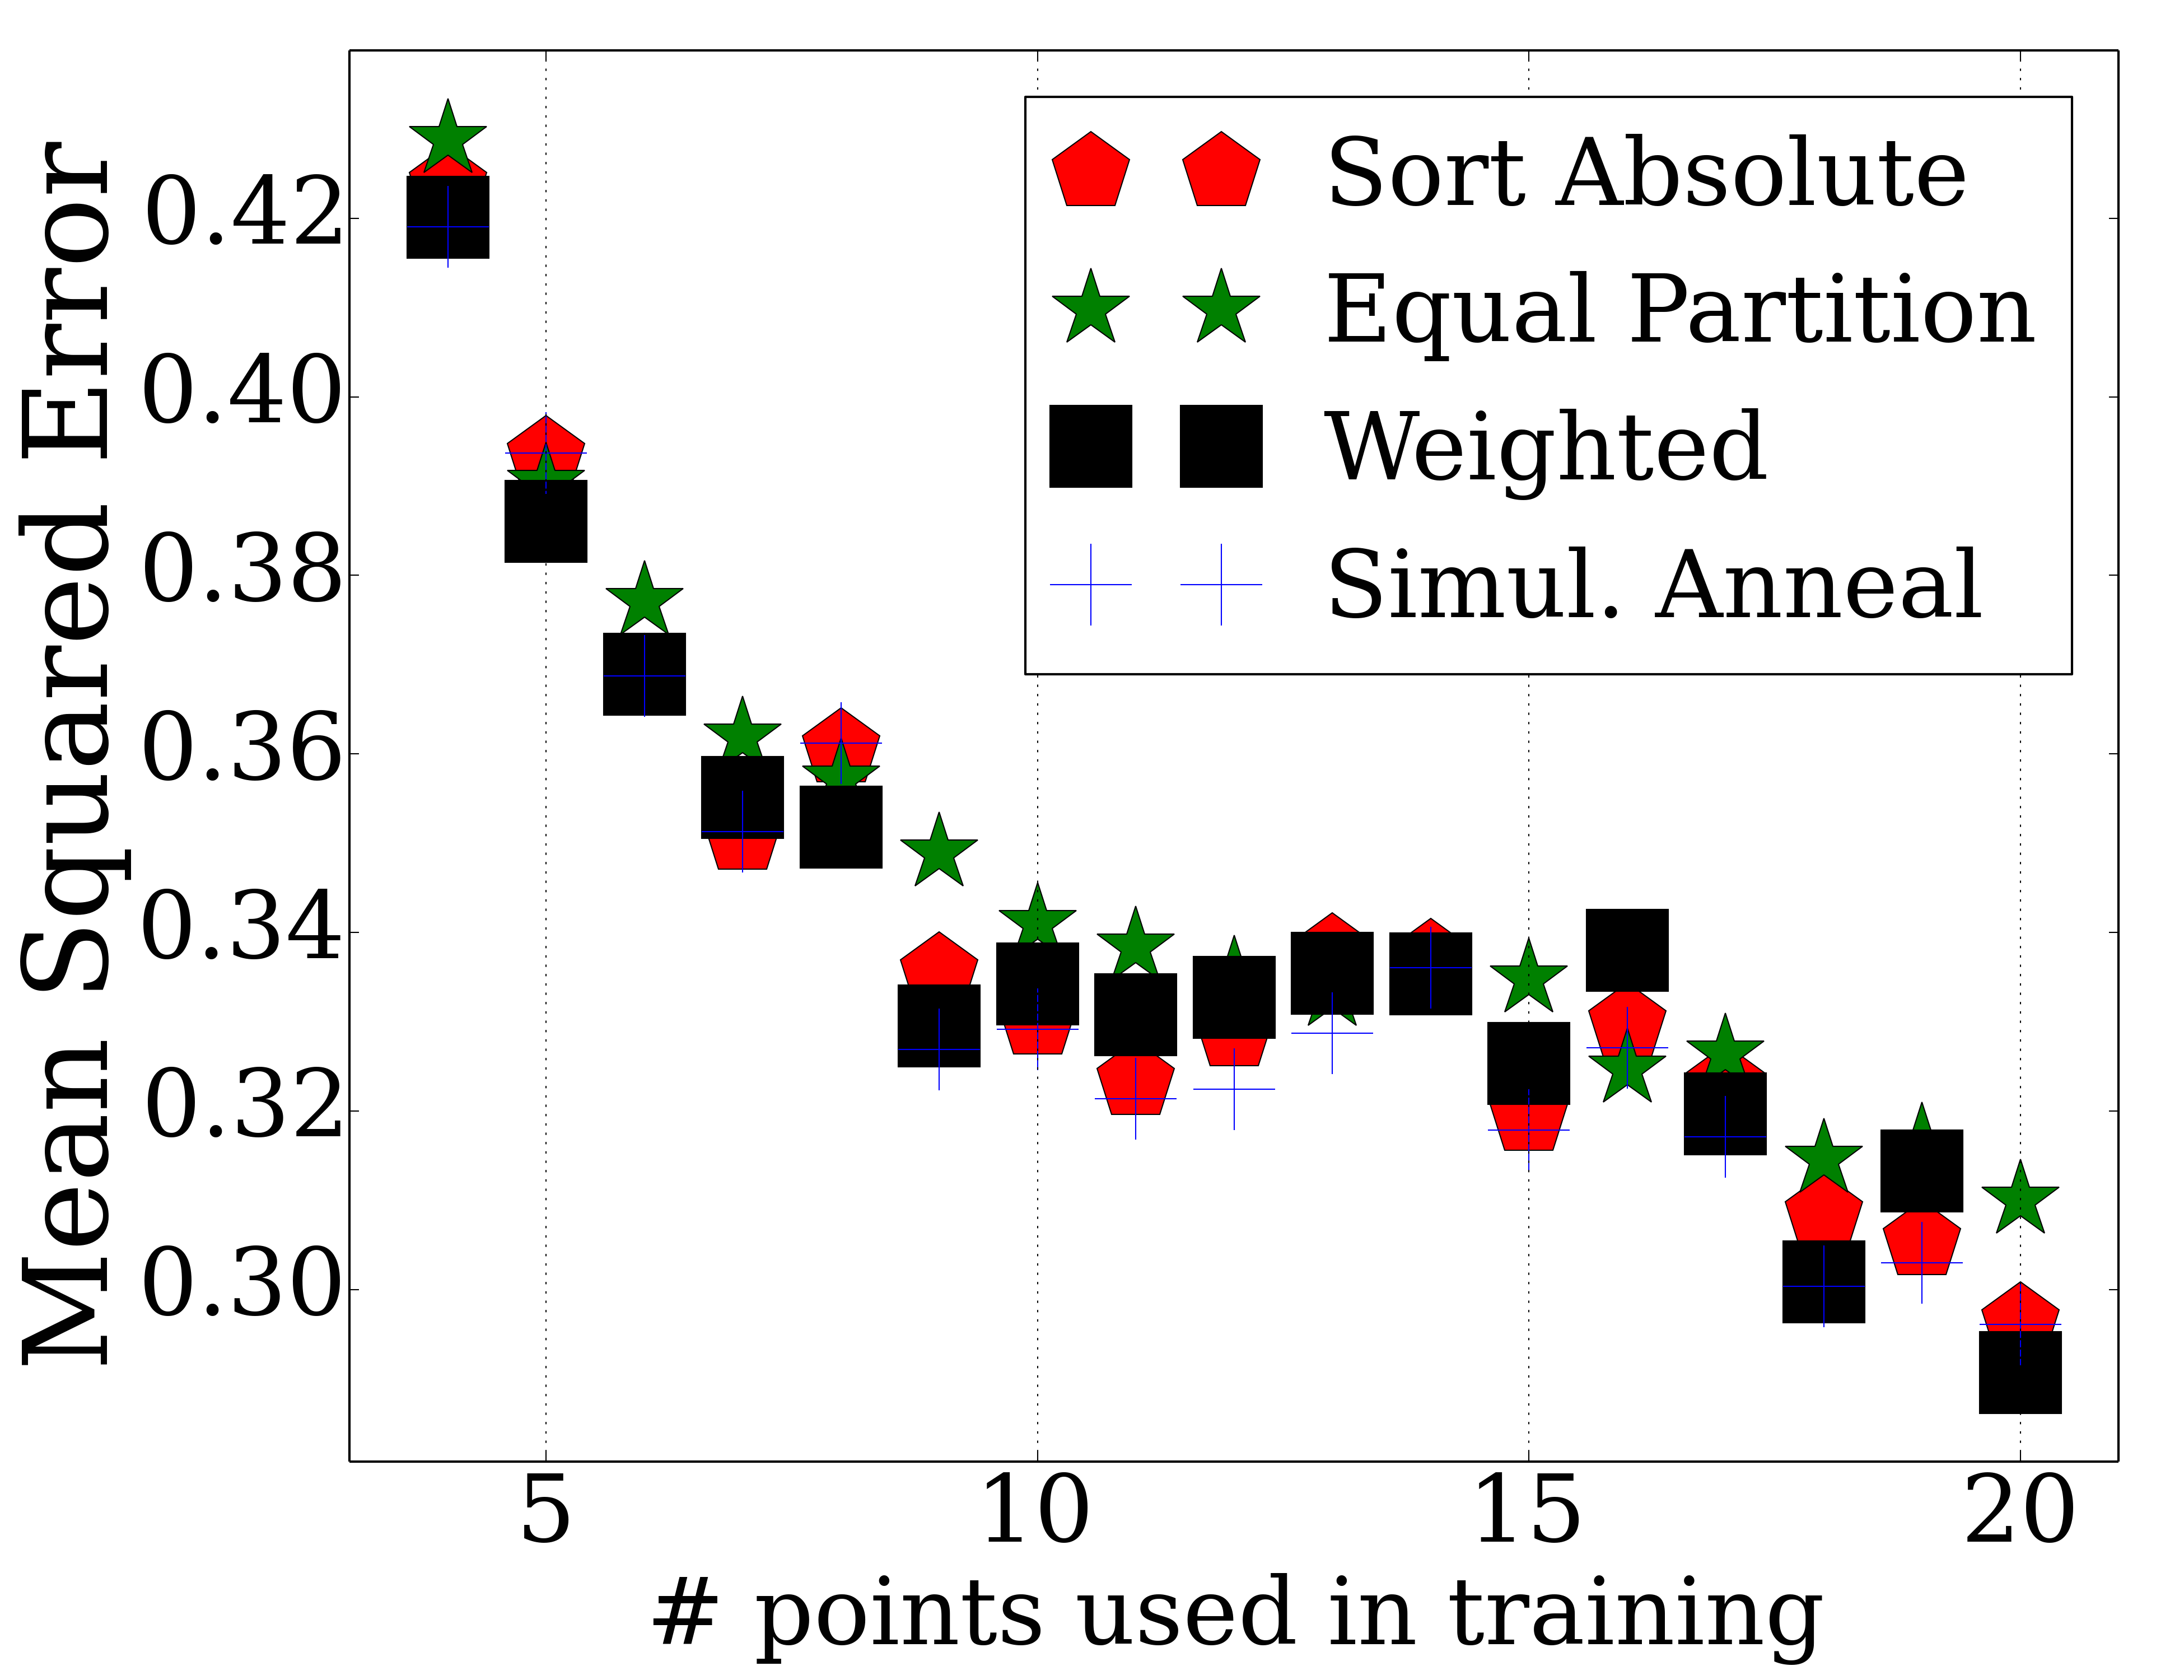
\includegraphics[scale=0.4]{../avgplot.png}
\caption{Performance in terms of Mean Squared Error}
\label{fig:fig1}
\end{figure}

% \section{Modeling by gaussian mixtures}

% In general, we try to fit the following function to expression data for gene $d$, $d_{g}$:
% %
% \begin{equation}\label{eq:mixture}
% d_{g}(t) \approx \sum_{t' \in T} \alpha_{t'}g^{\sigma}_{t'}(t)
% \end{equation}
% %
% where $\alpha_{t'}$ is the mixture coefficient for gaussian kernel centered at $t'$ and $g_{t'}(t) = \exp^{-\frac{(t-t')^{2}}{2\sigma^{2}}}$ is the corresponding gaussian kernel. Here, we use gaussian kernel for $g_{t'}$, but other parametric forms may be used as well.

% \subsection{Known $\sigma^{2}$}

% When variance $\sigma^{2}$ is known for each kernel, problem of learning the $k$-subset of most informative time points becomes convex. Additionally, existing lasso path solvers such as Least Angle Regression~(LARS)~\cite{efron2004} returns the whole solution path with the same complexity of finding a solution for a single regularization parameter.

% Among the returned solution path, we select the solution which has the number of $k$ nonzero time points. In practice, finding a solution with exactly $k$ nonzero points is not guaranteed, so we greedily remove the time point with the least increase in the error from the closest larger solution if exact $k$ nonzero point solution does not exist. In this case, we may even assume that $k$ is not provided, and select the best $k$ by Bayesian Information Criterion~(BIC)~\cite{bic}. We observe that using same variance for each time point may lead to a poorer performance, so we assume a nonuniform $\sigma^{2}$ for each time point and estimate it heuristically as follows: For each time point, we find its optimal $\sigma$ that minimizes the sum of absolute deviation of the predicted and true expression values of all the remaining points.  

% \subsection{Unknown $\sigma^{2}$}

% When $\sigma^{2}$ is unknown, optimization problem is not convex anymore so we follow an iterative two-step approach as follows: In the first step, we optimize for the best $\sigma$ given mixture coefficients $\alpha$s. In the second step, we solve for the best $\alpha$'s given $\sigma$ estimated in the first step. Both steps are convex. We also have a l$2$ regularization for $\alpha$'s. Optimization at each step can be solved quite fast by quasi-newton method L-BFGS~\cite{liu1989}. Regularization parameter is selected by $5$-fold cross-validation as the one which minimizes the prediction errors. We iterate both steps $5$ times.

% \section{Modeling The Subset Selection as an Infinite Dimensional Regression}
% %by Combinatorial Search over Smoothing Splines}

% This section is still in progress.  

% In the most general case, we do not assume any parametric form for kernel in Equation~\ref{eq:mixture} where our problem becomes similar to infinite-dimensional regression. However, the difficulty is that estimating both kernels and $\alpha$'s simultaneouly is coupled. In order to decouple their estimation, we should use more complicated majorization minimization type methods~\cite{zhou2013}. We add a regularization term for selecting smooth kernels as well as a l$1$ regularization term selecting a sparse subset of $\alpha$'s.

% When estimating $g^{\sigma}_{t'}(t)$ by majorization minimization method, we will solve Euler-Lagrange equations.

% \section{Modeling Multiple Genes Simultaneously}

% This section is still in progress.

% We will extend our proposed solutions to multiple genes. In this case, we should also decide the number of gene clusters and our solution must also include a step for assigning genes to clusters. Model parameters will be defined for each cluster instead of each single gene.

% \section{Single gene prediction performance}

% We plot the gene expression prediction performance for two genes~(TCF12, IGF1) independently as in Figures~\eqref{fig:res1}--\eqref{fig:res4}. 
% In general, the prediction performance starts to increase quickly after a number of time points. We do not see a major improvement by unknown variance compared to the known case suggesting the quality our heuristic.

% \begin{figure}[!h]
% \begin{minipage}{1.0\textwidth}
% \subfloat[Mean Absolute Error]{\label{fig:res1}\includegraphics[width=0.48\columnwidth]{error_tcf12.png}}
% \hfill
% \subfloat[Pearson]{\label{fig:res2}\includegraphics[width=0.48\columnwidth]{pearson_tcf12.png}}
% \hfill \\
% \centering{A) TCF12} \\
% \subfloat[Mean Absolute Error]{\label{fig:res3}\includegraphics[width=0.48\columnwidth]{error_igf1.png}}
% \hfill
% \subfloat[Pearson]{\label{fig:res4}\includegraphics[width=0.48\columnwidth]{pearson_igf1.png}}
% \hfill \\
% \centering{B) IGF1}
% \end{minipage}
% \caption{Gene-expression prediction of A) TCF12, B) IGF1 genes in terms of mean absolute error and pearson correlation $\rho$.}
% \end{figure}

% We also select the time points by TCF12, and fit a cubic smoothing spline over the same points for IGF1 by selecting regularization parameter via $5$-fold cross-validation. Figures~\eqref{fig:res5}--\eqref{fig:res6} show the performance in terms of mean absolute error and pearson correlation respectively.

% \begin{figure}[!h]
% \begin{minipage}{1.0\textwidth}
% \subfloat[Mean Absolute Error]{\label{fig:res5}\includegraphics[width=0.48\columnwidth]{error_inter.png}}
% \hfill
% \subfloat[Pearson]{\label{fig:res6}\includegraphics[width=0.48\columnwidth]{pearson_inter.png}}
% \hfill
% \end{minipage}
% \caption{Predicting the gene expression of TCF12 by learning subset of time points for IGF1.}
% \end{figure}

\bibliographystyle{splncs03} 
\bibliography{predict}

\end{document}